
\section{Overall Approach}
\label{sec:overall-approach}

The overall approach was to apply a hierarchy of \emph{secure} state machines to describe the patrol
base operations and verify them in the ACL and HOL.  To do this, it was focused on two things:
translating the patrol base operations from the Ranger Manual \cite{rangerhandbook} into the hierarchy of state machines
and then verifying these in the access-control logic (ACL) using the Higher Order Logic (HOL)
theorem prover.  These two tasks are described separately in this section.

\section{The Hierarchy of \emph{Secure} State Machines}
\label{sec:hier-emphs-state}

We applied the principle of complete mediation to the patrol base operations using a hierarchy
of \emph{secure} state machines.  Our decision was guided by the following logic.  First, a hierarchy
of \emph{secure} state machines was a simple framework for abstracting the patrol base operations into
levels.  Each level added a layer of complexity.   Each layer of complexity included more details
about the patrol base operations.  Second, the hierarchy of \emph{secure} state machines was easy to
modularize.  Each level of abstraction was modularized and each \emph{secure} state machine within a
particular level was modularized.  Third, the principle of complete mediation was implicit in
the \emph{secure} state machine structure.    Finally, the hierarchy of \emph{secure} state machines could
build-off of previous HOL implementations.  A \emph{secure} state machine theory in HOL already existed
and was tested.   This was the ssm11 parameterizable \emph{secure} state machines.  We modified this
theory and used it.  \\

The patrol base operations were clearly defined in the Ranger Manual \cite{rangerhandbook}  and the security principles
were embedded within these definitions.  But, the patrol base operations were not defined with the
principle of complete mediation in mind.  To adapt the operations, we first abstracted them into six
states (or phases): planning state (PLAN_PB), move to the operational rally point (ORP) (MOVE_TO_ORP),
conduct ORP operations (CONDUCT_ORP), move to the patrol base (MOVE_TO_PB), conduct the patrol base
operations (CONDUCT_ORP), and complete the patrol base operations (COMPLETE_PB).  These six states
and the transitions among them comprised the top-level state machine. A first draft of the top-level
abstraction was shown in figure 1.1.\\\\\\\\\\\\\\\\\\\\\\\\\\\\

\begin{figure}[h]
  \centering
  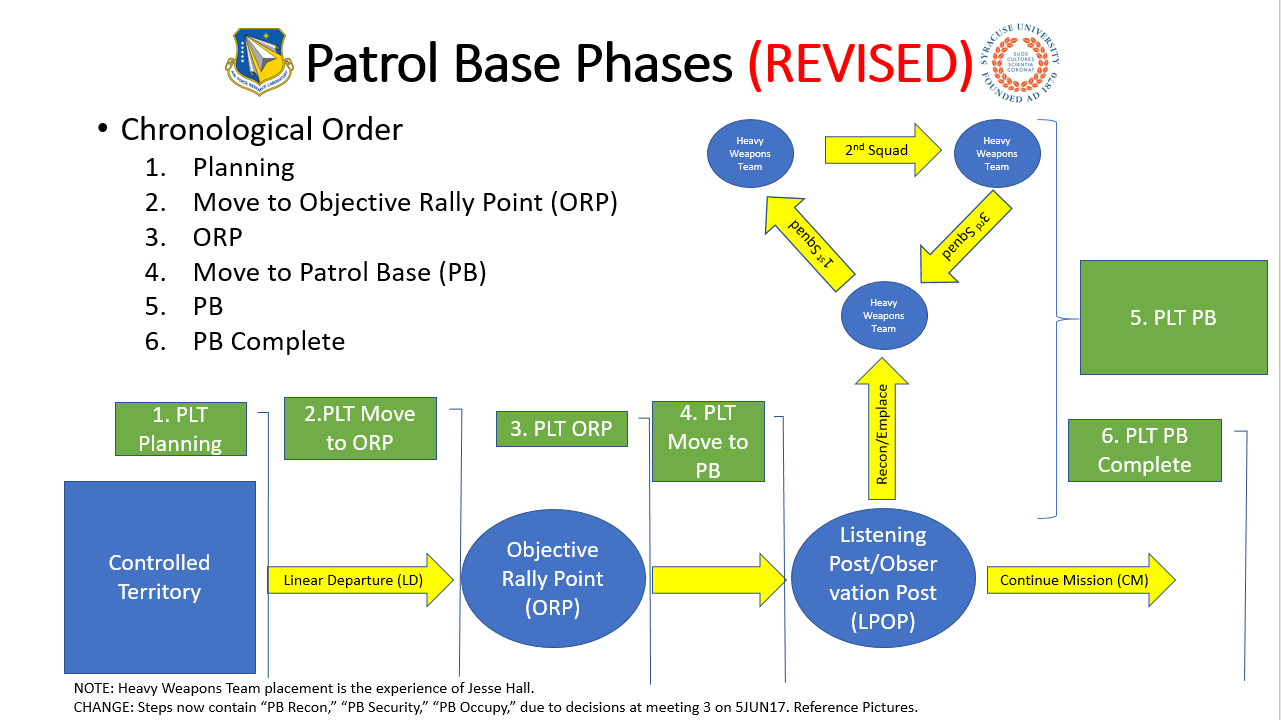
\includegraphics[width=0.7\linewidth]{map31.png}
  \caption{First separation of the patrol base operations into phases.}
\end{figure}

We transformed this top-level state machine into a \emph{secure} state machine in order to apply the
principle of complete mediation.  The principle of complete mediation applied to the patrol base
operations required that we verify the authentication and authority of all principals making request
to access objects (for the patrol base operations, objects were states and their transitions).
For the top-level state, we defined principals and their authorities.  The top-level \emph{secure}
state machine had only one principal, the Platoon Leader, who had the authority to request transitions
among all states in the top-level \emph{secure} state machine.   Figure 1.2 showed a diagram of the
top-level \emph{secure} state machine.

\begin{figure}[h]
  \centering
  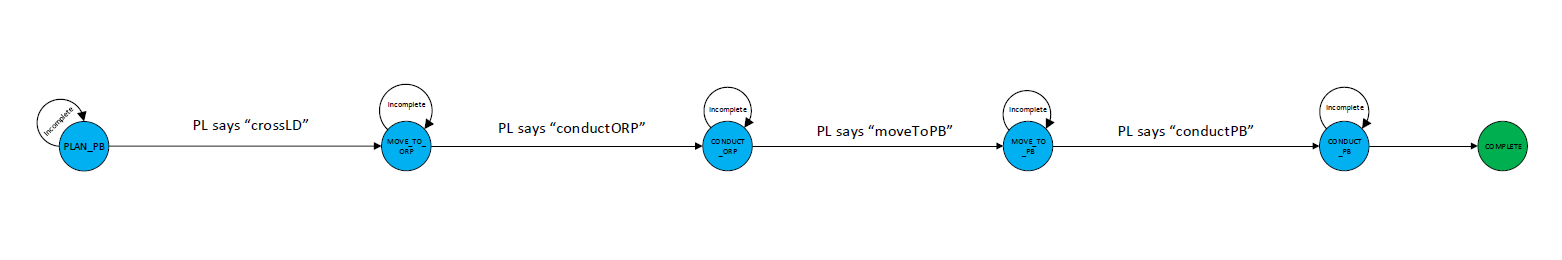
\includegraphics[width=1\linewidth]{map32.png}
  \caption{Top-level \emph{secure} state machine diagram}
\end{figure}

The top-level \emph{secure} state machine states were themselves made into \emph{secure} state machines. These
\emph{secure} state machines were called the sub-level \emph{secure} state machines.  Figure 1.3  showed the
top-level and sub-level \emph{secure} state machines.  The top-level states were colored dark blue and
sub-level states were colored light blue.  The end-state for the top-level was colored green. The
red circles were "escape states" which were not verified at the time of this documentation and
remain for future work.  Transitions among states were denoted with lines connecting two states.
Commands to execute transitions were written above the lines.  \\\\\\\\\\\\\\\\\\\\\\

\begin{figure}[h]
  \centering
  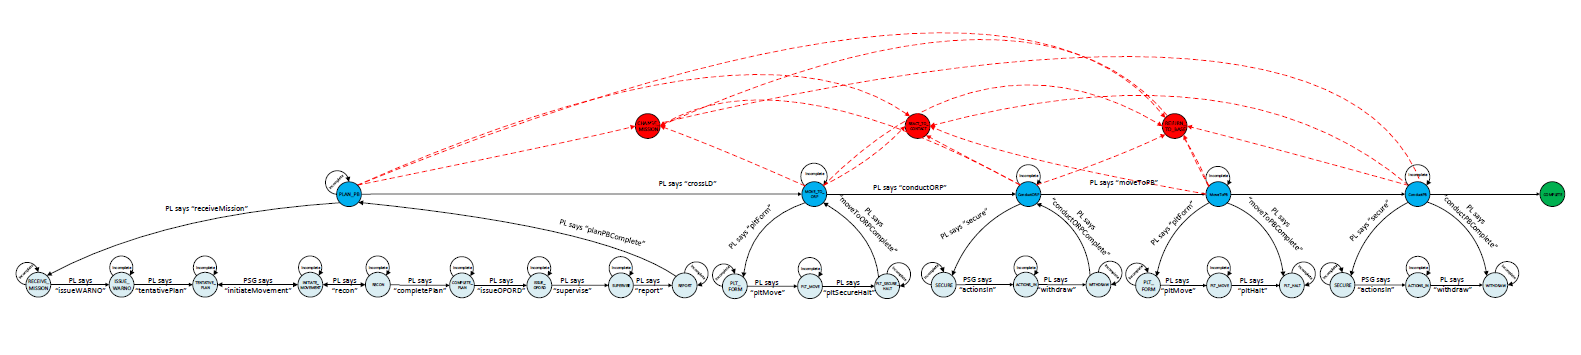
\includegraphics[width=1\linewidth]{map34.png}
  \caption{Top-level and sub-level \emph{secure} state machine diagram.}
\end{figure}

Each state in the top-level \emph{secure} state machine (except for the end state) was made into a
\emph{secure} state machine at the sub-level.  That is, each sub-level \emph{secure} state machine
was a state in the top-level \emph{secure} state machine. (The details are described in more detail
in the results section.)  These sub-level \emph{secure} state machines were described at a lower
level of abstraction.  An example of one of these sub-level states was shown in figure 1.4.  This is
the PlanPB sub-level \emph{secure} state machine.  It had nine states.  In the diagram, the three
states outlined in orange were non-sequential.  That is, the order of transition was irrelevant.
But, all three states had to be complete before transitioning to the next COMPLTE_PLAN state. The
other states were to be executed sequentially.  This \emph{secure} state machine had two principals
Platoon Leader and Platoon Sergeant.  Each of these principals was granted authority to over transitions
for a subset of states as denoted in the diagram.

\begin{figure}[h]
  \centering
  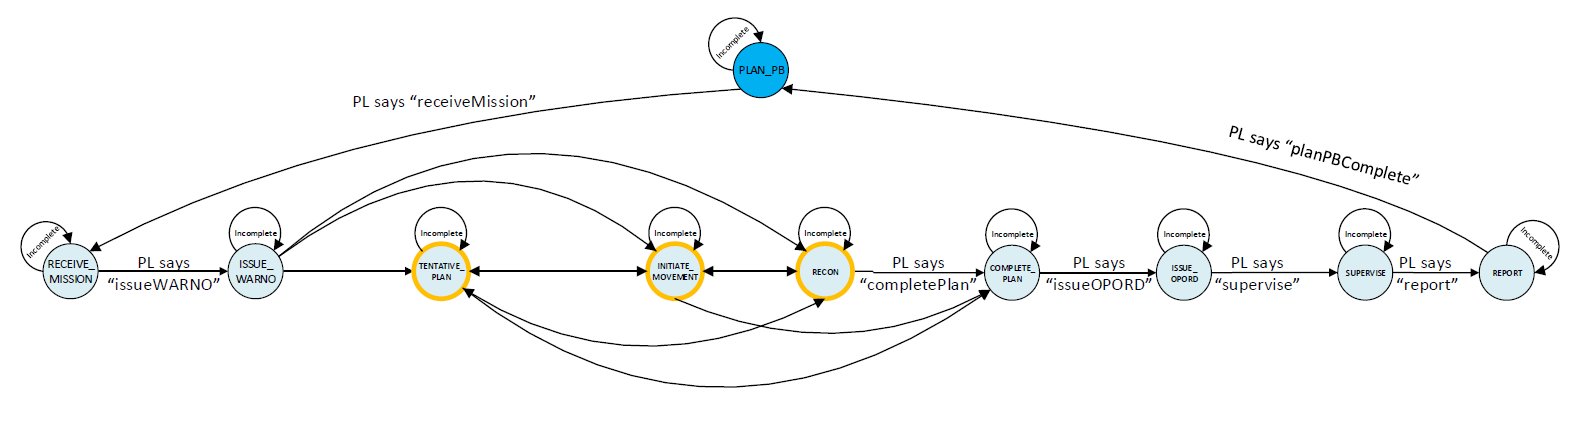
\includegraphics[width=1\linewidth]{map36.png}
  \caption{One of the sub-level \emph{secure} state machine diagram.}
\end{figure}

A vertical slice through the whole of the patrol base operations was translated from the Ranger Manual.
Figure 1.5 showed the diagram.  The diagram elements were too small to read clearly on this page, but
the diagram provided an overview of the scope of the project.  Similar to the top-level and sub-level
\emph{secure} state machines, the sub-sub-level \emph{secure} state machines were formed from the states
at the sub-level.  These \emph{secure} state machines were discussed in detail but not verified in HOL
at the time of this documentation.  Additional theories to indicate platoon and solider readiness were
discussed also but not verified in ACL and HOL. These theories are also described in more detail in the
Future Work and Research section.

\begin{figure}[h]
  \centering
  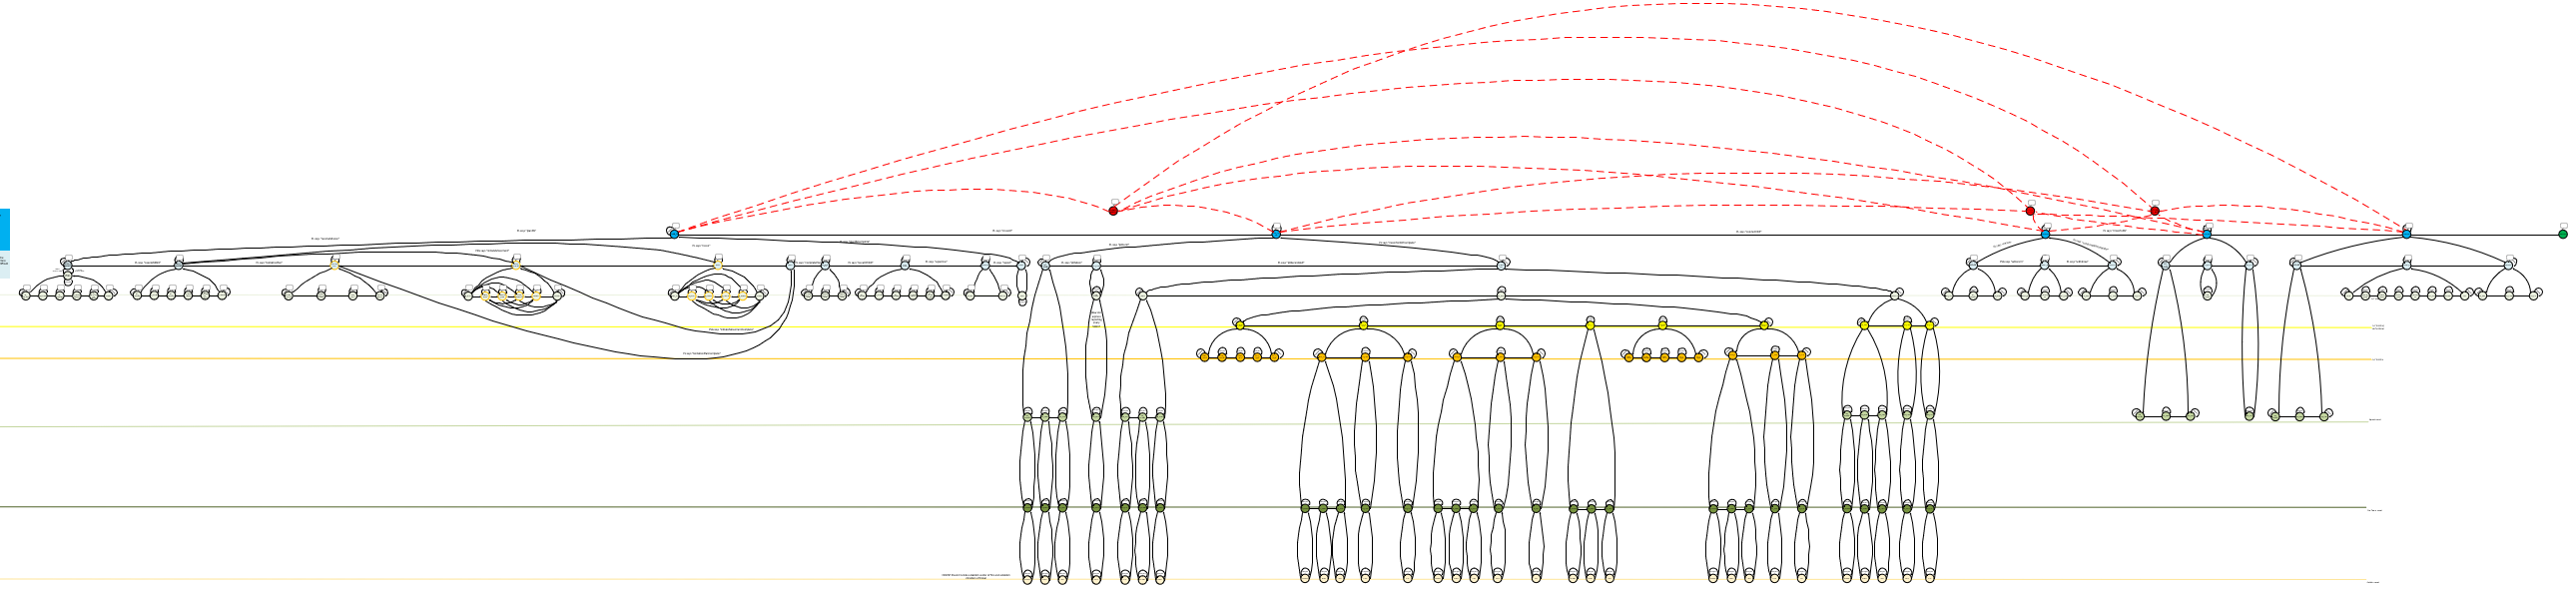
\includegraphics[width=1\linewidth]{map37.png}
  \caption{Hierarchy of secure state machines.}
\end{figure}


\section{ACL and HOL Verification}
\label{sec:acl-hol-verification}

The access-control logic (ACL) was defined in the text \emph{Access Control, Security, and Trust:
  A Logical Approach} \cite{acst}.  The theories were verified in HOL by who ? and used for this project.
These theories were acl_infRules, and satListTheory.   These theories were used to build the
parameterizable \emph{secure} state machines (ssm11 and ssm), \emph{secure} state machines, and
supporting theories.  ssm11 was defined and verified prior to this project by who ?  and modified
for this project.   ssm was modified from ssm11 based on discoveries in this project.  Both ssm11
and ssm were described in more detail in the context of their use in the Results section.   The
\emph{secure} state machines (i.e., top-level and sub-level \emph{secure} state machines) and
supporting theories (i.e., *TypeScript.sml) were defined and verified specifically for this project
and were discussed in more detail in the Results section.  \\

The version of HOL used was HOL-4 [Kananaskis 11  (stdkml, built Sat Aug 05 19:17:00 2017)]
running on  PolyML, version ?.  HOL was run in the Unix environment on Ubuntu (version 16.04.3 LTS)
on Oracle's Virtual Box (version 5.1.26r117224 (Qt5.6.2)).  CVS (version 1.12.13 MirDebian-11) was
used to coordinate file sharing among the contributors of this project. EmitTeX was used to generated
pretty-printed documentation of the HOL code.  This code was included in the appendix T. \\

To compile the theories in HOL and generate the EmitTeX pretty-printed pdf file, we ran the following code from inside the folder ABD/HOL/HOLReportsOMNI.

\begin{itemize}
\item Open a terminal in ABD/HOL/HOLReportsOMNI
\item execute "Holmake cleanAll"
\item execute "make clean"
\item execute "Holmake"
  \item execute "make"\\
  \end{itemize}

  To generate the EmitTeX pretty-printed documentation in each of the HOLReports folders we ran the following code
  \begin{itemize}
  \item Open a terminal in ABD/HOL/HOLReportsOMNI
  \item execute "Holmake cleanAll"
    \item execute "Holmake"\\\\
    \end{itemize}

    To compile all the HOL code in the folder we ran the following from the HOL subfolder of ABD.
    \begin{itemize}
    \item execute "Holmake cleanAll"
    \item execute "make clean"
    \item execute "Holmake"
      \item execute "make"\\
      \end{itemize}

\section{Patrol Base Operations Translations}
\label{sec:patr-base-oper}




% ---- this points LaTeX to PatrolBaseDoc.tex ----
% Local Variables:
% TeX-master: "../PatrolBaseDoc"
% End: